\documentclass[conference]{IEEEtran}
\usepackage{amsmath,amssymb,graphicx,booktabs,url}
\title{Independent-Sensor Traffic Speed Forecasting\\with Temporal Tree Ensembles: A Phase 1 Study}
\author{\IEEEauthorblockN{Team T072, Section C}
\IEEEauthorblockA{Rudraksh Sharma, Anshuman Mehta, Vridhi Chaudhary,\\Bineet Keshari, and Kavya Katal}}
\begin{document}
\maketitle
\begin{abstract}
We implement a reproducible machine-learning pipeline for forecasting traffic speed independently at road sensors. Persistence and a training-only historical average are compared with multi-output Random Forest and direct-horizon XGBoost. The inspected METR-LA file has 34,272 five-minute observations at 207 sensors. Causal features, purged chronological partitions, missing-target masks and run manifests support comparison on common targets at horizons from five to sixty minutes. Parameters are selected on a small validation pilot. The previously inspected test interval is reported as exploratory, not a pristine holdout. This is a forecasting study; no graph neural network or signal controller is implemented.
\end{abstract}
\begin{IEEEkeywords}
traffic speed, forecasting, Random Forest, XGBoost, chronological validation
\end{IEEEkeywords}

\section{Problem and Related Work}
The broader faculty allocation is Multi-Agent Traffic Flow Control via Graph Attention Networks and LWR Models. This Phase 1 addresses independent-sensor speed forecasting; graph learning and simulated control remain future work.

At forecast origin $t$, sensor $i$ supplies history $v_{t-11:t,i}$ and known calendar information $c_t$. Predict
\begin{equation}
\hat v_{t+h,i}=f_{i,h}\bigl(\phi(v_{t-11:t,i},c_t)\bigr),\quad h=1,\ldots,12.
\end{equation}
Here $\phi$ is causal feature construction. Twelve observations end at $t$ and begin $55$ minutes earlier. Offsets 3, 6 and 12 mean 15, 30 and 60 minutes ahead. Random Forest shares one estimator across horizons for each sensor; XGBoost fits a direct estimator for each sensor/horizon.

Seasonal univariate traffic modeling motivates temporal structure \cite{williams}; work on typical and atypical traffic conditions motivates period-specific analysis \cite{castro}. Random Forest \cite{breiman} and XGBoost \cite{chen} provide non-neural nonlinear models. Forecast-metric limitations \cite{hyndman} motivate several error measures. DCRNN \cite{li} provides benchmark provenance and future spatial-learning motivation. Its published scores are not equivalent-protocol comparisons with our purged prototype. Accessible bibliographic, abstract and method sources were checked; independent replication of these papers is not claimed.

\section{Data and Quality}
The inspected matrix has 207 sensor columns at five-minute spacing from 1 March to 27 June 2012. The benchmark describes speed in mph; units are not supplied by the loader itself. There are no separate measured flow or occupancy channels in this matrix, and none are fabricated. Speed, flow, density and occupancy are distinct physical quantities.

Under the benchmark policy, zero and NaN targets are excluded from scoring. Infinite or negative raw speeds are rejected. Missing inputs are causally filled and flagged; targets are never imputed. Actual-file checksums, sensor order, boundaries, missingness and outage statistics accompany the run. Constructed distance-kernel adjacency matches the supplied graph reference but is not used by the prediction models.

The upstream repository code is MIT-licensed; separate raw-data redistribution rights remain unverified, so datasets are excluded from delivery. Timezone/daylight-saving semantics are unresolved. Calendar and peak labels refer to recorded clock values; deployment-time local-clock claims are therefore inappropriate.

\begin{figure*}[t]
\centering
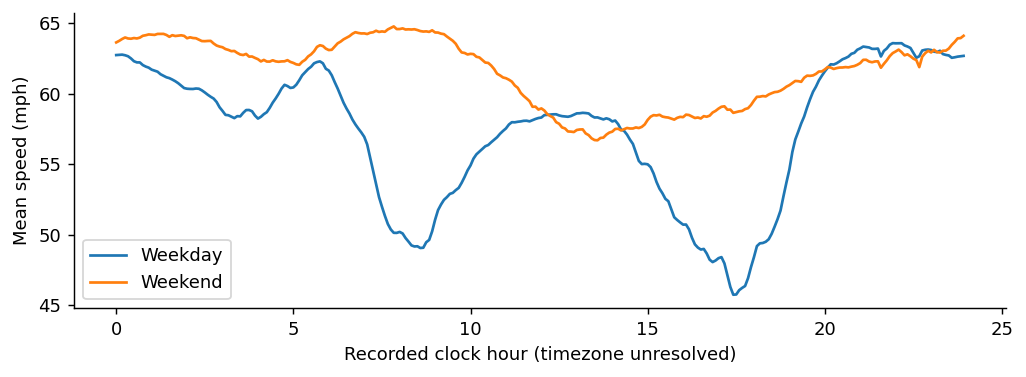
\includegraphics[width=.92\textwidth]{images/daily_profile.png}
\caption{Training-only daily profiles; clock timezone is unresolved.}
\end{figure*}

\section{Methodology}
\subsection{Partitioning and Leakage Prevention}
Nominal anchor proportions are 70/10/20. Validation retains two prototype halves: tuning and a separately reported second interval; no stacker is trained. Removing the final eleven anchors of each earlier partition ensures its targets end no later than the next partition's first forecast origin. Retained counts are 23,963 training, 1,701 tuning, 1,702 second-validation and 6,850 test anchors. Previously observed input history may cross a boundary.

Fit medians and historical averages only within the retained training interval. Tree training uses every second retained anchor to bound compute; evaluation retains the full anchor grid. Both learned models receive the same candidate training anchors, but their valid-label rules differ.

Baseline test outputs were examined before this extension. Parameters are selected only on tuning data, then frozen. Subsequent test comparisons remain exploratory. Renaming exposed observations would not create an independent holdout.

\subsection{Causal Features}
The 38 features are twelve speed lags, twelve original missingness flags, three trailing means, history standard deviation/minimum/maximum, two differences, missing fraction, sine/cosine of time of day/week, and a weekend flag. Fill proceeds left to right inside each history; leading gaps use the training median. Statistics use the explicitly filled history. No scaler or target-derived historical-profile feature is used.

\subsection{Reference Methods}
Persistence repeats the latest valid history value; an entirely missing window uses the historical-average fallback. Historical average groups training readings by sensor and time-of-week slot, then falls back to time-of-day and overall sensor averages. These distinguish immediate continuity from recurring structure.

\subsection{Random Forest}
Each sensor-specific forest averages regression trees and jointly outputs twelve future values. Bootstrap sampling occurs only inside training; it is not a random evaluation split. A training row with any missing future label is excluded under the joint-output rule. This may skew learning away from outage periods; exclusion counts are retained. Parameters control ensemble size, depth, minimum leaf size and feature fraction.

\subsection{XGBoost}
Each sensor/horizon gets a separate boosted-tree regressor and excludes that horizon's invalid labels only. Its objective has a loss and a tree-complexity penalty,
\begin{equation}
\mathcal L=\sum_j\ell(y_j,\hat y_j)+\sum_k\Omega(f_k).
\end{equation}
Learning rate, depth, minimum child weight and subsampling constrain complexity. Two predefined configurations per method are compared by valid-point MAE at headline horizons on six evenly spaced sensor indices in the tuning interval. Actual parameters/objective are in the manifest. This budgeted pilot is not exhaustive optimization. Sparse-label cases use a predeclared, counted historical-average fallback.

\section{Evaluation and Observed Results}
With valid-target error $e=\hat v-v$,
\begin{align}
\mathrm{MAE}&=\tfrac1n\sum |e|,\\
\mathrm{RMSE}&=\sqrt{\tfrac1n\sum e^2},\\
\mathrm{MAPE}&=\tfrac{100}{n}\sum |e/v|.
\end{align}
MAE/RMSE use speed units; MAPE uses percent and remains unstable near zero. Missing/zero targets are masked identically across methods. Metrics pool valid sensor-time points by horizon and retain valid counts. Peak periods are provisional weekday clock hours 07:00--10:00 and 16:00--19:00.

\begin{table}[t]
\centering
\caption{Exploratory test errors on the common target grid. Lower is better; these are not classification accuracies.}
\resizebox{\columnwidth}{!}{\begin{tabular}{llrrr}
\hline
Method & min & MAE & RMSE & MAPE (\%) \\
\hline
M0 persistence & 15 & 3.48 & 6.37 & 8.57 \\
M0 persistence & 30 & 4.17 & 7.98 & 10.77 \\
M0 persistence & 60 & 5.32 & 10.25 & 14.39 \\
M1 ha & 15 & 4.19 & 7.85 & 13.03 \\
M1 ha & 30 & 4.19 & 7.85 & 13.03 \\
M1 ha & 60 & 4.19 & 7.85 & 13.03 \\
M3 rf & 15 & 2.97 & 5.44 & 8.07 \\
M3 rf & 30 & 3.42 & 6.37 & 9.81 \\
M3 rf & 60 & 3.90 & 7.25 & 11.71 \\
M4 xgb & 15 & 2.92 & 5.78 & 8.04 \\
M4 xgb & 30 & 3.38 & 6.91 & 10.06 \\
M4 xgb & 60 & 3.87 & 7.99 & 12.59 \\
\hline
\end{tabular}
}
\label{tab:metrics}
\end{table}

\begin{figure*}[t]
\centering
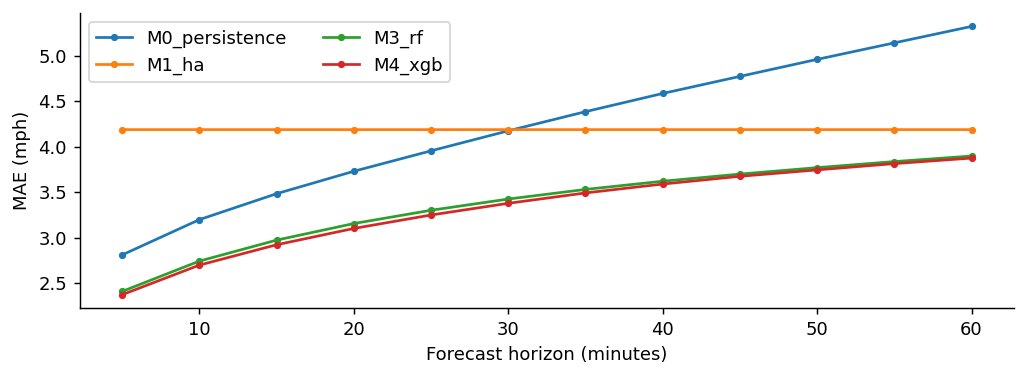
\includegraphics[width=.92\textwidth]{images/mae_horizons_test.png}
\caption{Observed error across all twelve future offsets.}
\label{fig:errors}
\end{figure*}

\begin{figure*}[t]
\centering
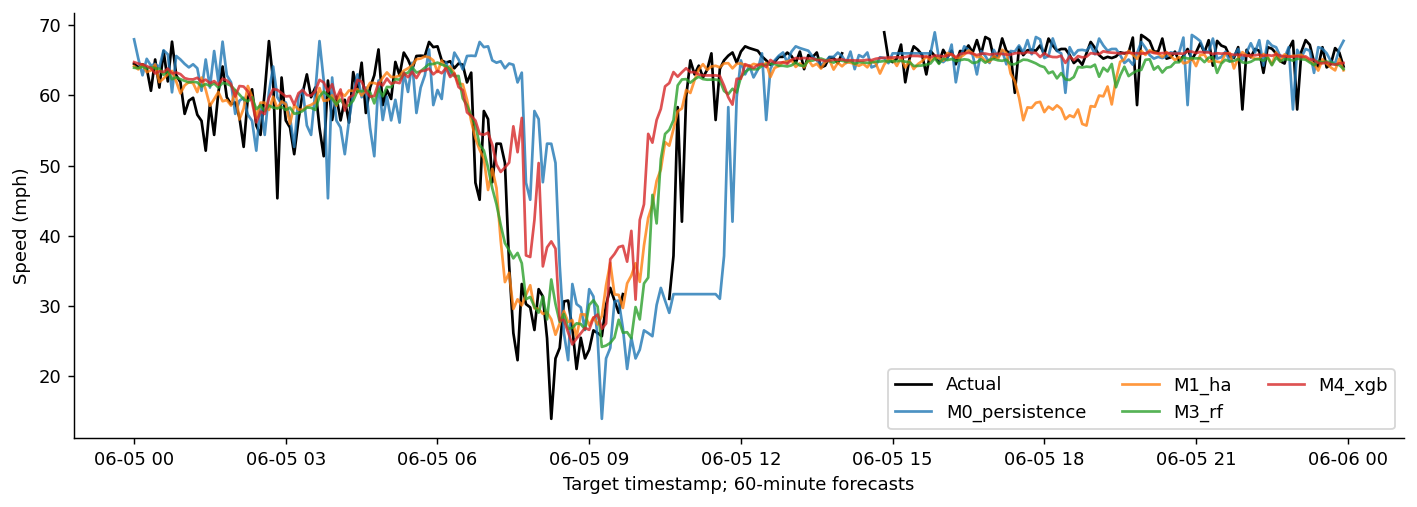
\includegraphics[width=.94\textwidth]{images/forecast_example.png}
\caption{A middle-index sensor on the second test day, selected by fixed index/date rather than by the best-looking model result. Forecasts are sixty minutes ahead.}
\end{figure*}

Table \ref{tab:metrics} and Fig. \ref{fig:errors} show measured outcomes, not target scores. Companion tables cover tuning, second validation, peak/off-peak, weekday/weekend and per-sensor errors. The generated results note records descriptive changes relative to persistence. Lowest aggregate error does not imply superiority at every sensor or period.

The exploratory Diebold--Mariano utility uses sensor-average loss differences per timestamp and a HAC variance estimate, with Holm adjustment across one declared pair's horizons. This weighting differs from point-pooled MAE when sensor availability varies. Dependence and prior test exposure limit inferential claims. No bootstrap confidence intervals are claimed. The raw XGBoost test tensor contains 24 negative predictions among 17,015,400 forecasts. They were retained rather than silently clipping test scores; a prospectively specified nonnegativity rule is a future improvement.

\section{Limitations and Traffic Theory}
Independent-sensor temporal features do not directly observe congestion at neighbouring links. The LWR conservation equation
\begin{equation}
\partial\rho/\partial t+\partial q/\partial x=0,\qquad q=\rho v
\end{equation}
motivates spatial propagation conceptually. Speed alone does not identify measured density/flow states or a calibrated shockwave speed. No LWR calibration, GAT superiority or control benefit is established.

Limitations include one region/historical period, a small tuning pilot, strided training, forest complete-label exclusion, exposed test results, unresolved timezone/data rights and MAPE sensitivity. Broader prospectively specified temporal validation and multi-seed stability remain future work. High accuracy is not guaranteed, and feature importance is association rather than causation.

\section{Reproducibility and Contributions}
Pinned dependencies, causal-feature/partition tests, source/data/config SHA-256 manifests, exact settings, runtime records, saved estimators, a prediction command and reproducible figures support inspection. Only trusted locally generated serialized artifacts should be loaded. Raw data, environments and model binaries are excluded from version control.

The project owner prepared this integrated implementation/report with substantial AI assistance, building on the supplied teammate prototype. Team names identify the roster, not evidence of individual module authorship. Contributions and assistance must be declared accurately. No individual's viva readiness is certified by a commit name.

\section{Conclusion}
This Phase 1 pipeline compares two references and two temporal tree methods under common targets and explicit chronology safeguards. Measured errors and documented limits support a concrete forecasting discussion. Spatial deep learning, flow calibration and simulated control are separate future tasks.

\begin{thebibliography}{6}
\bibitem{breiman} L. Breiman, Random forests, \emph{Machine Learning}, 45, 5--32, 2001.
\bibitem{chen} T. Chen and C. Guestrin, XGBoost: A scalable tree boosting system, \emph{KDD}, 2016, doi:10.1145/2939672.2939785.
\bibitem{williams} B. M. Williams and L. A. Hoel, Modeling and forecasting vehicular traffic flow as a seasonal ARIMA process, \emph{Journal of Transportation Engineering}, 129(6), 664--672, 2003.
\bibitem{castro} M. Castro-Neto et al., Online-SVR for short-term traffic flow prediction under typical and atypical traffic conditions, \emph{Expert Systems with Applications}, 36, 6164--6173, 2009.
\bibitem{hyndman} R. J. Hyndman and A. B. Koehler, Another look at measures of forecast accuracy, \emph{International Journal of Forecasting}, 22(4), 679--688, 2006.
\bibitem{li} Y. Li et al., Diffusion convolutional recurrent neural network: Data-driven traffic forecasting, \emph{ICLR}, 2018, arXiv:1707.01926.
\end{thebibliography}
\end{document}